% Source : http://tex.stackexchange.com/questions/23647/drawing-a-directory-listing-a-la-the-tree-command-in-tikz

\documentclass[parskip,14pt]{scrartcl}
	\usepackage[margin=15mm]{geometry}
	\usepackage{tikz}

	\newcounter{treeline}

	\newcommand{\treeroot}[1]{% Title
		\node[above] at (0,0) {#1};%
		\setcounter{treeline}{0}
	}

	\newcommand{\treeentry}[2]{% Title, Level
		\draw[->] (#2-1,-\value{treeline}/2) -- (#2-1,-\value{treeline}/2-0.5) -- (#2+0.5,-\value{treeline}/2-0.5) node[right] {#1};
		\stepcounter{treeline}
	}

	\newcommand{\altentry}[2]{% Title, Level
		\draw[->] (#2-1,-\value{treeline}/2) -- (#2-1,-\value{treeline}/2-0.5) -- (#2+0.5,-\value{treeline}/2-0.5) node[right] {#1};
		\foreach \x in {1,...,#2}{%
			\draw (\x-1,-\value{treeline}/2) -- (\x-1,-\value{treeline}/2-0.5);
		}
		\stepcounter{treeline}
	}


\begin{document}

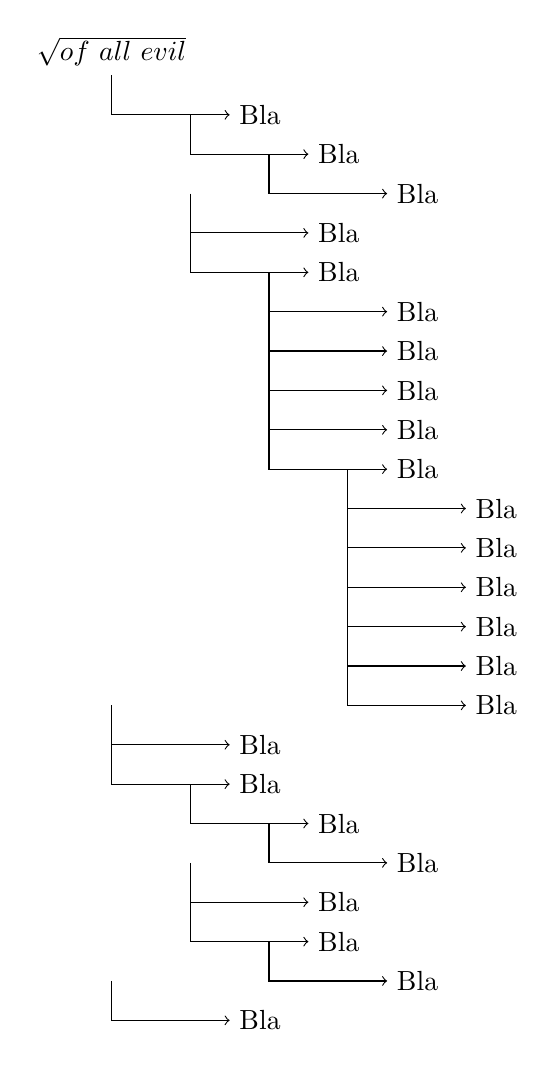
\begin{tikzpicture}
	\treeroot{$\sqrt{of\ all\ evil}$}
	\treeentry{Bla}{1}
		\treeentry{Bla}{2}
			\treeentry{Bla}{3}
		\treeentry{Bla}{2}
		\treeentry{Bla}{2}
			\treeentry{Bla}{3}
			\treeentry{Bla}{3}
			\treeentry{Bla}{3}
			\treeentry{Bla}{3}
			\treeentry{Bla}{3}
				\treeentry{Bla}{4}
				\treeentry{Bla}{4}
				\treeentry{Bla}{4}
				\treeentry{Bla}{4}
				\treeentry{Bla}{4}
				\treeentry{Bla}{4}
	\treeentry{Bla}{1}
	\treeentry{Bla}{1}
		\treeentry{Bla}{2}
			\treeentry{Bla}{3}
		\treeentry{Bla}{2}
			\treeentry{Bla}{2}
		\treeentry{Bla}{3}
	\treeentry{Bla}{1}
\end{tikzpicture}

\hspace{2cm}

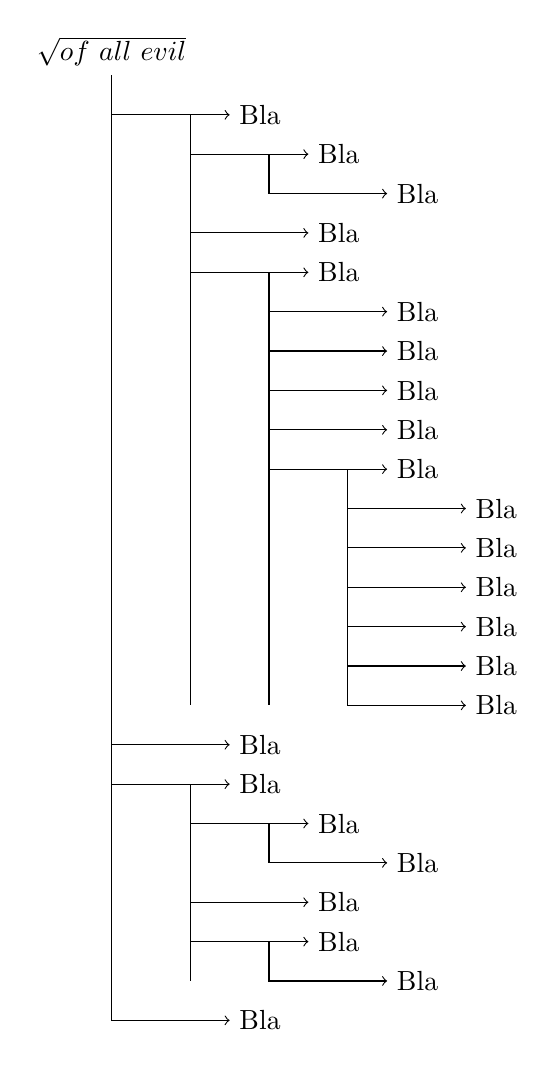
\begin{tikzpicture}
	\treeroot{$\sqrt{of\ all\ evil}$}
	\altentry{Bla}{1}
		\altentry{Bla}{2}
			\altentry{Bla}{3}
		\altentry{Bla}{2}
		\altentry{Bla}{2}
			\altentry{Bla}{3}
			\altentry{Bla}{3}
			\altentry{Bla}{3}
			\altentry{Bla}{3}
			\altentry{Bla}{3}
				\altentry{Bla}{4}
				\altentry{Bla}{4}
				\altentry{Bla}{4}
				\altentry{Bla}{4}
				\altentry{Bla}{4}
				\altentry{Bla}{4}
	\altentry{Bla}{1}
	\altentry{Bla}{1}
		\altentry{Bla}{2}
			\altentry{Bla}{3}
		\altentry{Bla}{2}
		\altentry{Bla}{2}
			\altentry{Bla}{3}
	\altentry{Bla}{1}
\end{tikzpicture}

\end{document}
